\chapter{Background}


\section{SynSemClass}

The SynSemClass lexicon \parencite{uresova-etal-2020-synsemclass} --- formerly CzEngClass --- is a multilingual event-type ontology currently under development. An event-type ontology is a hierarchy of classes that denote events and states. Each class is populated by class members --- words. Unrelated to our work, the SynSemClass project also seeks to link the classes and its members to a plethora of existing lexical resources, such as the EngVallex \parencite{EngVallex20}, CzeEngVallex \parencite{czengvallex}, FrameNet \parencite{ruppenhofer2016framenet}, PropBank \parencite{kingsbury2002treebank} and many others. The lexicon currently consists of words from English, Czech, German and Spanish. See \cref{fig:synsemclass-scheme} for the scheme of the lexicon and \cref{fig:synsemclass-tools} for the tools used to view the ontology data. The goal of this bachelor thesis is to explore machine learning methods as preprocessing steps to automatically suggest annotations for extending the ontology into a new language.

\begin{figure}[h]
\centering
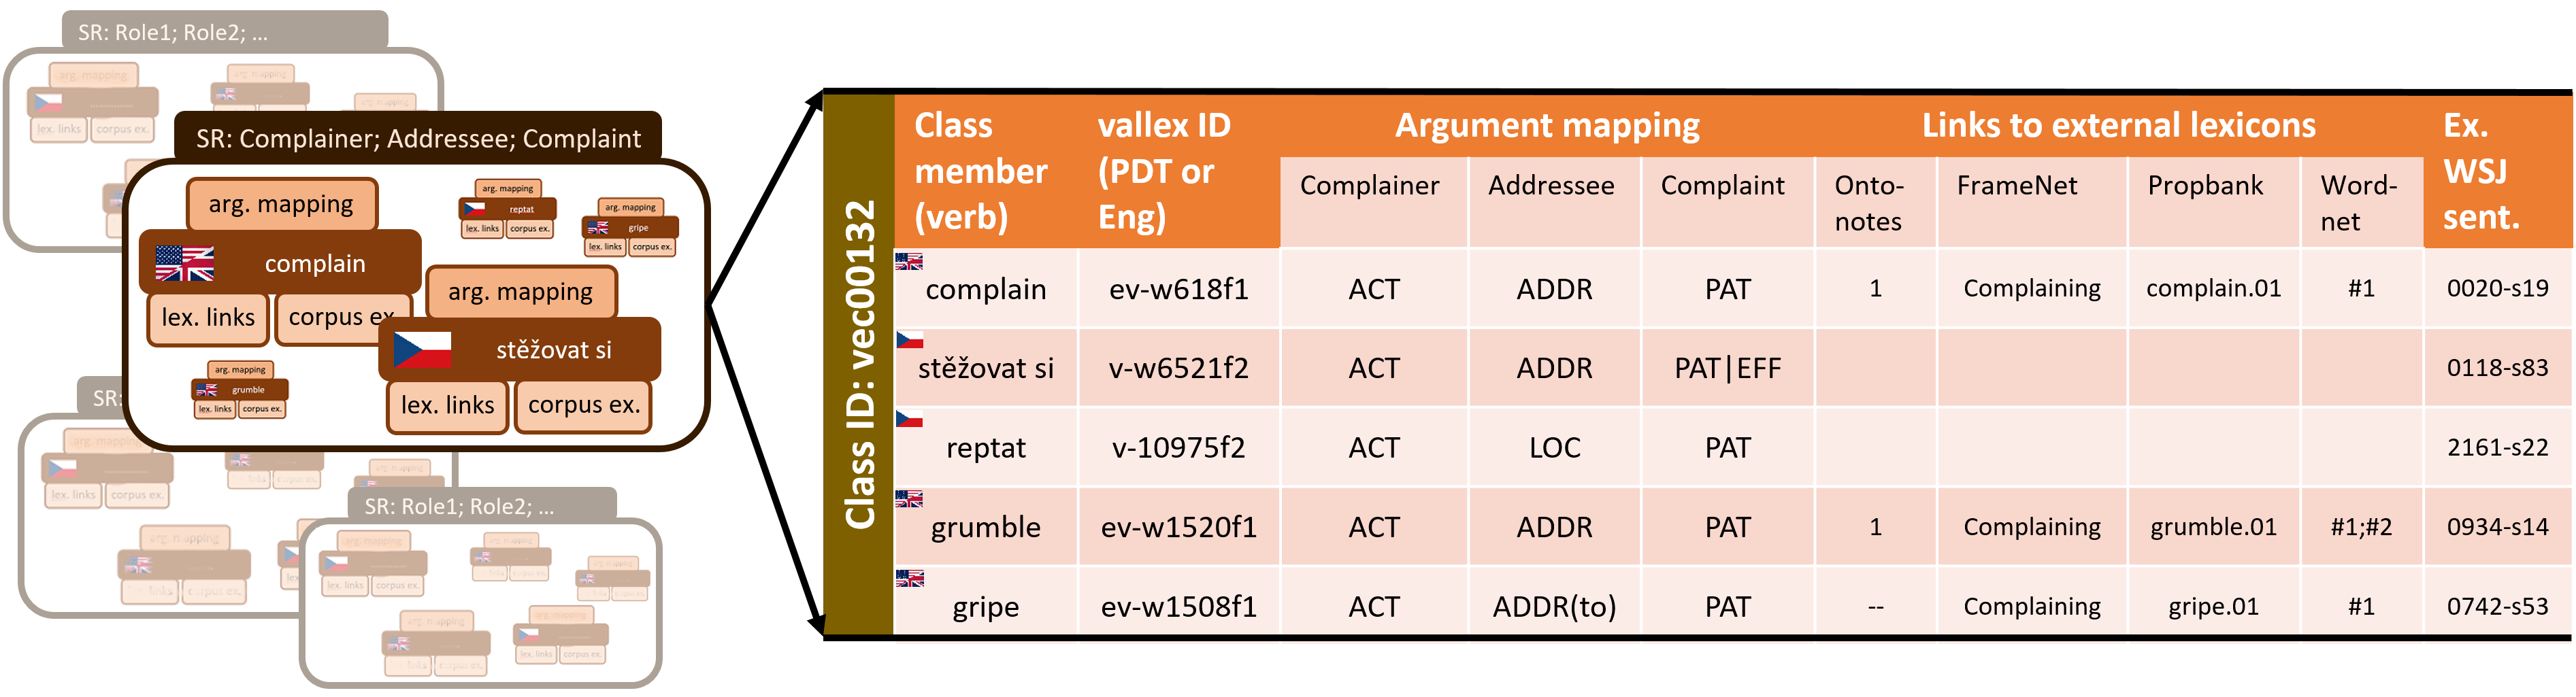
\includegraphics[width=0.9\linewidth]{img/06-final-ssclass-scheme}
\caption{The overall scheme of the SynSemClass lexicon and an example of a class (“complain-stežovat si”) \parencite{uresova-etal-2020-synsemclass}.}
\label{fig:synsemclass-scheme}
\end{figure}

In the rest of this section, we briefly summarize the initial annotation process of the ontology. We focus only on the steps that are relevant to us and omit the rest.

\citet{ssc_start} built the first Czech and English version of the lexicon by semi-randomly choosing Czech verbs of various frequencies from the Prague Czech-English Dependency Treebank (PCEDT) \parencite{pcedt} and letting those be the names and seeds of new classes. They used automatic word alignment to get the English counterparts. Manual pruning and annotation followed. The PCEDT corpus contains an annotation layer relating to semantics and deep syntax, the so called tectogrammatical layer. \citet{ssc_start} used this information to build the links to other resources as well as other linguistic annotation, which we will not delve into, as it does not affect our work. 

German was added by \citet{uresova-etal-2022-making} by automatically word-aligning the English-German part of the ParaCrawl \parencite{banon-etal-2020-paracrawl} corpus. They decided on a set of English verbs, for which they found the most common German alignments. These were then manually filtered and annotated for correct classes. As they did not use a part-of-speech tagger, they could not distinguish between verb and noun forms of the verb (e.g., `to run' vs. `a run') and these cases had to be manually removed.

\begin{figure}[t]
\centering
\begin{subfigure}[t]{0.49\textwidth}
\centering
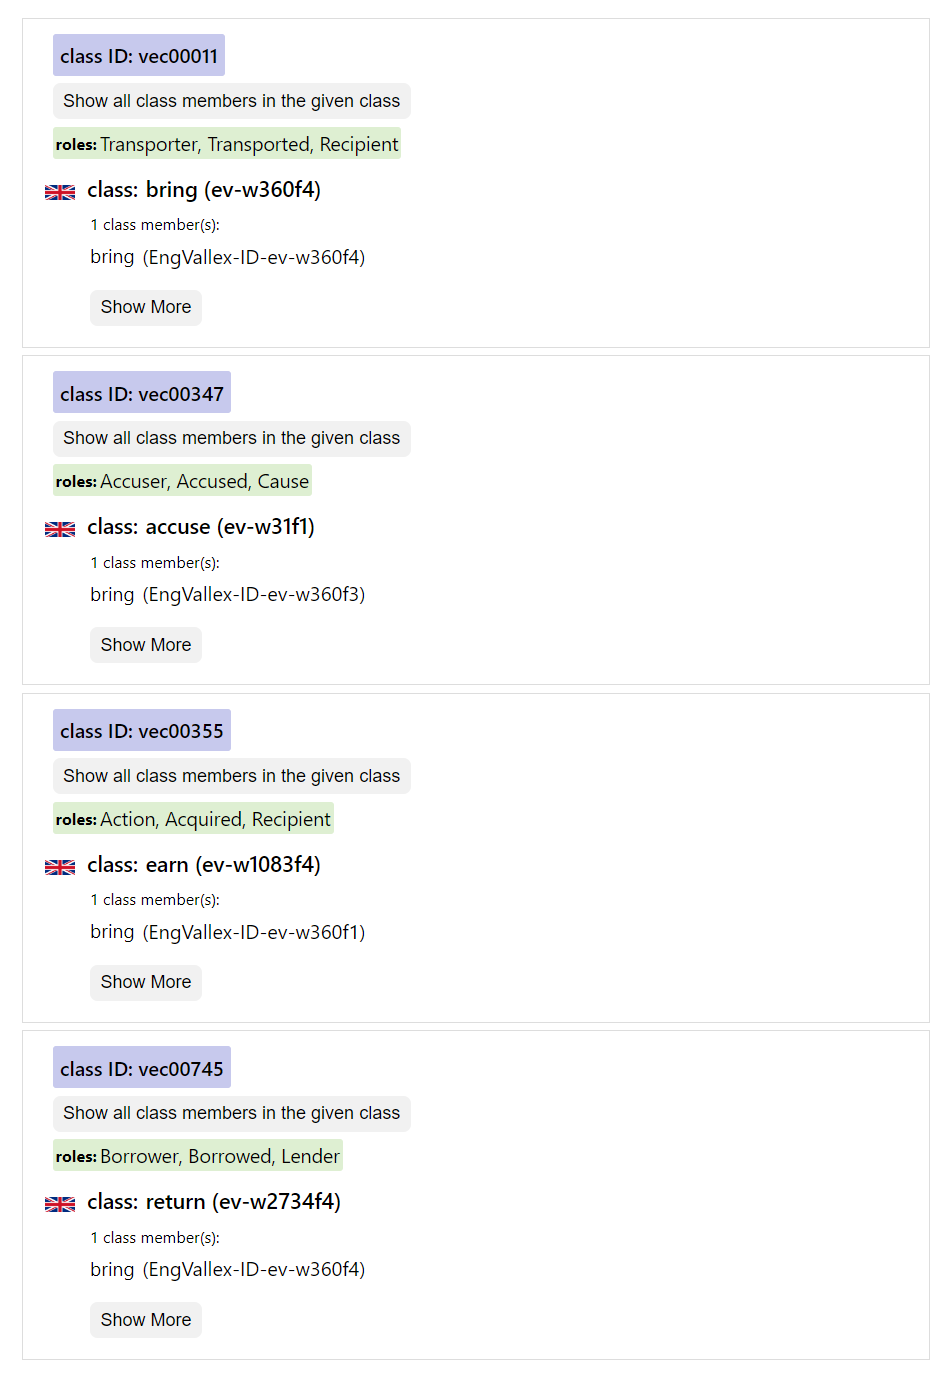
\includegraphics[width=0.9\linewidth]{img/synsemclass_tool}
\caption{A lookup of the word `bring' in the SynSemClass Search\footnotemark tool shows that it belongs into multiple classes.}
\label{fig:synsemclass-search}
\end{subfigure}\hfill
\begin{subfigure}[t]{0.49\textwidth}
\centering
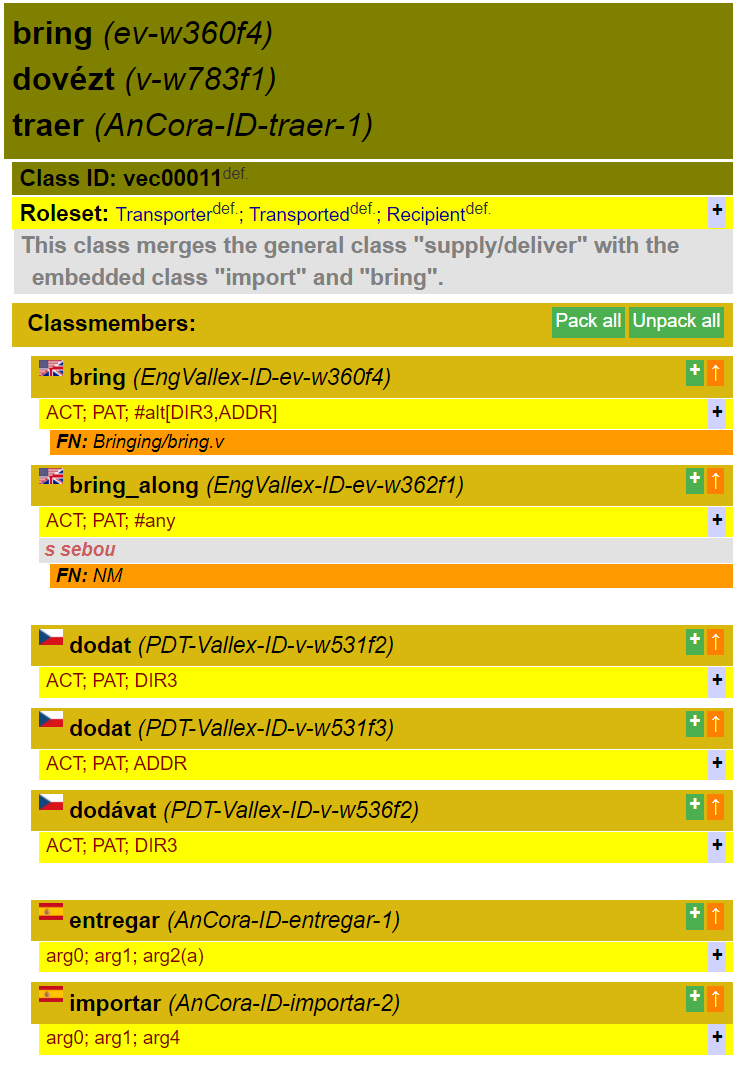
\includegraphics[width=0.9\linewidth]{img/synsemclass_class}
\caption{The class with ID vec00011 has several words associated with it as shown in the browse tool.\footnotemark}
\label{fig:synsemclass-browse}
\end{subfigure}
\caption{Two different tools for the SynSemClass ontology. Note that both results are trimmed.}
\label{fig:synsemclass-tools}
\end{figure}

\addtocounter{footnote}{-1}
\footnotetext{\url{https://lindat.mff.cuni.cz/services/SynSemClassSearch/}}
\addtocounter{footnote}{1}
\footnotetext{\url{https://lindat.cz/services/SynSemClass50/SynSemClass50.html}}

The Spanish part \parencite{SSC_Spanish} was built in a similar manner to German, using automatic word alignment on parallel data. Additionally, they used semantic information extracted from a Spanish lexical resource, AnCora \parencite{taule-etal-2008-ancora}, to perform automatic filtering. Although AnCora contains only Spanish lemmas, it links to several English resources that are also linked in the SynSemClass ontology. If the automatic alignment created alignments for which semantic data was linkable to AnCora but the senses did not match, the pairing was discarded. Unlike the German team, they had data tagged for part of speech.

There is a key difference between the initial phases of the SynSemClass annotation and the challenge of a new language presented here. In the initial phases of the SynSemClass annotation, more extensively annotated resources were available, including (automatically) word-aligned parallel corpora and manually annotated verb senses with respective valency dictionaries. In our case, the starting point is simply a sentence-aligned parallel corpus between a newly added language and a source language already annotated in the corpus, without any additional semantic information or a valency lexicon in the target language. Our language of choice is Korean. We describe Korean as well as our motivation behind choosing it in the next section.

We note that this work was done on SynSemClass 4.0\footnote{\url{https://lindat.mff.cuni.cz/repository/xmlui/handle/11234/1-4746}}. The current version of SynSemClass is 5.0\footnote{\url{https://lindat.mff.cuni.cz/repository/xmlui/handle/11234/1-5230}}.


\section{Korean language}

We chose Korean as the language on which we test our methods for adding a completely new language into the ontology, as well as the overall design of the ontology to accommodate a non-European language. The author has a lower-intermediate knowledge of Korean, however, we would like to acknowledge that the work has not been checked by anyone either fluent in the language or with a sufficient linguistic background in it. We are confident that any errors made are of low significance and not damaging to the work as a whole. What follows is a brief introduction to the Korean language and its grammar.

Korean is an East Asian language spoken by more than 75 million people, most of whom live on the Korean peninsula. While being similar to Japanese in many aspects, the languages are generally regarded as not related and Korean is attributed its own language family, the Koreanic language family, whose only other member is the Jeju language, spoken by about 5,000 speakers on the island Jeju south of the Korean peninsula. Efforts trying to link Korean and Japanese are complicated by previous use of writing systems based on the Chinese writing system, which can obscure historic pronunciation. In 1443, Korean king Sejong the Great invented and later published a new, more phonemic, script. However, due to resistance from scholars and the upper classes, the script became widely adopted only in the second half of the 20th century.

Nowadays, the Korean script is called Hangul \ort{한글} (with a different name used in North Korea). Depending on the way one counts, it uses 24-51 letters (complex letters are considered to be made of basic letters, however they may have vastly different pronunciation, e.g., ㅏ /a/ + ㅣ /i/ = ㅐ /e/). The letters have mnemonic shapes, see \cref{fig:korean-k} for an example.


\begin{wrapfigure}{r}{0.3\textwidth}
\includesvg[width=0.9\linewidth]{img/korean_k.svg}
\caption{The Korean letter \ort{ㄱ} /k/ is based on the placement of the tongue on the velum. \mbox{Image} adapted from \citet{velar-plossive}.}
\label{fig:korean-k}
\end{wrapfigure}

Similar letters have similar shapes unlike most of the Latin alphabet (e.g., compare the Latin pair \ort{g} \ort{k} and the very roughly equivalent pair in Hangul \ort{ㄱ} \ort{ㅋ}). Hangul letters are arranged into blocks, which consist of three positions for letters --- initial, medial and an optional final position. For example, the letters ㅎ /h/ + ㅏ /a/ + ㄴ /n/ can form the block 한 /han/. For the rest of the work, we will use the Revised romanization system as reference, while also providing the Hangul counterpart.

Korean is an agglutinative language. Agglutination is the process of adding (often multiple) morphemes to a stem of a word, with the stem mostly remaining unchanged. To demonstrate the essence of this process and its difference from inflection, we will try to give an extreme example. It is not typical for a word to have this many morphemes, but it is not rare. \vspace{0.8em}

\begin{tabular}{llll}
성공 & seong-gong  &  & success \\
적 & jeog &  & “ful”, affix meaning of having such character \\
이 & i &  & be \\
었 & eoss &  & past tense \\
다고 & dago &  & quotation \\
\addlinespace
말했다 & malhaessda & & said \\
\addlinespace
\addlinespace
\multicolumn{4}{l}{성공적이었다고 말했다.} \\
\multicolumn{4}{l}{seong-gongjeogieossdago malhaessda.} \\
\multicolumn{4}{l}{`(He) said (he) was successful.'} \\
\end{tabular}
\vspace{0.8em}

In the above example, both subjects are omitted. Without context, it is unclear who said it and who was successful. This phenomenon is called pro drop (pronoun dropping). On top of dropping the subjects as is done in Slavic languages, Korean also allows for dropping of objects thanks to a phenomenon known as topic drop. The common phrase for `I love you.' \ortx{사랑해}{saranghae} does not say who loves whom. An example conversation would be: \vspace{0.8em}

\begin{tabular}{llll}
이 & i  &  & this \\
케이크 & ke-ikeu  &  & cake \\
좋아 & joh-a  &  & good \\
\addlinespace
누가 & nuga  &  & who \\
만들었어 & mandeur-eoss-eo  &  & made \\
\addlinespace
\addlinespace
\multicolumn{4}{l}{이 케이크 좋아. 누가 만들었어?} \\
\multicolumn{4}{l}{i keikeu joh-a. nuga mandeur-eoss-eo?} \\
\multicolumn{4}{l}{`This cake is good. Who made (it)?'} \\
\end{tabular}
\vspace{0.8em}

In Korean, the Subject-Object-Verb (SOV) word order is used, as opposed to English, Czech, German and most European languages, which usually use the Subject-Verb-Object (SVO) word order. This means that typically in a sentence, the subject comes first, followed by the object and the verb being the very last in the sentence.\vspace{0.8em}

\begin{tabular}{llll}
나는 & naneun  &  & I \\
사람 & saram  &  & person \\
만났다 & mannassda &  & met \\
\addlinespace
\addlinespace
\multicolumn{4}{l}{나는 사람 만났다.} \\
\multicolumn{4}{l}{naneun saram mannassda.} \\
\multicolumn{4}{l}{`I met a person.'} \\
\end{tabular}
\vspace{0.8em}

The change in word order is also present elsewhere, most notably in relative clauses, which come before the word they are modifying.\vspace{0.8em}

\begin{tabular}{llll}
바나나 & banana & & banana \\
준 & jun & & gave \\
그 & geu & & that  \\
사람 & saram & & person \\
만났다 & mannassda &  & met \\
\addlinespace
\addlinespace
\multicolumn{4}{l}{바나나 준 그 사람 만났다.} \\
\multicolumn{4}{l}{banana jun geu saram mannassda.} \\
\multicolumn{4}{l}{`(I) met that person who gave (me) a banana.'} \\
\end{tabular}
\vspace{0.8em}

We hope this section was sufficient in giving a very basic overview of the Korean language and its distinction from European languages. We will provide more examples of Korean grammar as they become relevant for the following sections.


\section{Related work}

The task of predicting a SynSemClass ontology class might seem to be the same as word sense disambiguation, but we note that the two tasks are different. \citet{word_sense_disambiguation} defines word sense disambiguation as selecting a single or more senses from a set of possible senses \textit{for the given word}, that is, each word has a different set of possible senses. With the SynSemClass ontology, each verb can be assigned to any of the circa 1000 SynSemClass classes. We cannot limit the scope of the senses simply based on the lemma. That is for several reasons.

Most importantly, the SynSemClass project allows for idiomatic meaning. For example, the expression `to lay the blame on someone' would be annotated the same as `to blame' / `to accuse' \parencite[section 4.3]{uresova-etal-2022-making}. Even if this were not the case, we assume the ontology is still under construction, so the full scope of a word's meaning is not known, either because the given language is only partially annotated, or because we are in the beginning of the process of adding the language to the ontology.

In the case of designing a completely new hierarchy of classes or (word) senses on a given set of words from scratch, unsupervised clusterization techniques have also been suggested, e.g., Brown clustering \parencite{brown-etal-1992-class}. However, our situation differs from such a setting. The ontology is already partially constructed, containing about 1000 classes, and the classes are partially populated with Czech, English, German and Spanish words that express the concepts of those classes. Our challenge is to incorporate words that possibly express the same concept(s) from an incoming new language into one or more of the existing classes or decide that no such class is relevant for the new word.
